\documentclass[times,10pt,twocolumn]{article}
\usepackage{latex8}
\usepackage{times}
\usepackage{graphicx}

\usepackage{amsmath}
\usepackage{tabularx}
\usepackage{booktabs}
\usepackage{colortbl}
\usepackage{tikz}
\usepackage{xcolor}
\usepackage{url}
\usepackage{balance}


\newcommand{\ub}{user defined-block}
\newcommand{\nPrograms}{250.166}
\newcommand{\nemptyPrograms}{14.285}
\newcommand{\nScriptPrograms}{233.514}

\newcommand{\numkids}{61~}
\newcommand{\lm}{\emph{Long Method}~}
\newcommand{\dup}{\emph{Duplication}~}

\newcommand{\todo}[1]{\textbf{#1}}



\begin{document}   

\title{Clones in Block-Based Languages: A Large Scale Analysis of Scratch Programs}

\author{Felienne Hermans\\
       {Delft University of Technology}\\
      {Mekelweg 4}\\
       {Delft, the Netherlands}\\
       {f.f.j.hermans@tudelft.nl}
}

\maketitle



\begin{abstract}
Recently, block-based programming languages like Alice, Scratch and Blockly have become popular tools for programming education. There is substantial research showing that block-based languages are suitable for early programming education. But do block-based programs suffer from code clones \emph{smelly} too? In a recent controlled experiment, we found that code clones in Scratch indeed hamper novice Scratch programmers. In this paper we explore how commonly code clones occur in Scratch. To that end we have scraped Scratch public repository and retrieved 250.000 programs. We have analyzed three types of clones within those programs': clones of entire scripts within sprites, clones of entire between sprites, and cloned conditions. We find that those clones occur in ... of programs.
\end{abstract}

\section{Introduction}

Scratch is a programming language developed to teach children programming by enabling them to create games and interactive animations. The public repository of Scratch programs contains over 12 million projects. Scratch is a \emph{block-based} language: users manipulate blocks to program. Block-based languages are visual languages, but also use some successful aspects of text-based languages such as limited text-entry and indentation, and as such are closer to `real', textual programming than other forms of visual programming, like dataflow languages are.

Block-based languages have existed since the eighties, but have recently found adoption as tools for programming education. In addition to Scratch, also Alice~\cite{conway_alice:_1994}, Blockly\footnote{\url{https://developers.google.com/blockly/}} and App Inventor~\cite{wolber_app_2011} are block-languages aimed at novice programmers.

In this paper we explore code clones smells in the context of block-based languages. \todo{hier nog wat background over clones, zie ICSE `13 uiteraard}

Clones so far have mostly been studied in the contact of object-oriented, textual source code, but some other directions have been taken, including spreadsheets and SimuLink programs. 

% Recently, it has been demonstrated that code smells occur in various alternative programming environments including spreadsheets~\cite{hermans_detecting_2012, hermans_detecting_2014}, Yahoo! Pipes~\cite{stolee_refactoring_2011} and LabView~\cite{chambers_smell-driven_2013}.
 
We ourselves have recently performed an experiment where we compared the performance of novice Scratch programmers between three 

Knowing that code clones can be harmful, we now turn to the question of whether they are common. As such, the goal of this paper is to \textbf{investigate whether code clones are common in public Scratch programs}.  To address this goal we have obtained \nPrograms~public Scratch programs by scraping the list of recent programs \todo{link}. We investigate three types of clones: clones of entire scripts within sprites, clones of entire between sprites, and cloned conditions.

The results show that \todo{todo}

The contributions of this paper are as follows:

\begin{itemize}
\item{A public data set of \nScriptPrograms~Scratch programs (Section \ref{dataset})}
\item{A clone Scratch detection algorithm with an open source implementation (Section \ref{algo})}
\item{An empirical evaluation of the occurrence of three types of clones in Scratch programs (Section \ref{results})}
\end{itemize}

\section{Background and Motivation}
\label{sec:background}
Block-based languages go back to 1986, when Glinert introduced the BLOX language~\cite{e._glinert_towards_1986}. BLOX consists of puzzle-like programming statements that can be combined into programs by combining them both vertically and horizontally. After a decade of little activity into block-based languages, they became a research topic again, starting with Alice~\cite{conway_alice:_1994}. More recently, new block-based languages have gained widespread popularity, especially powered by Scratch~\cite{resnick_scratch:_2009} and Blockly\footnote{\url{https://developers.google.com/blockly/}}. Over 100 million students have tried Blockly via Code.org, and the Scratch repository currently hosts over 12 million projects. Unlike in BLOX, in these new block-based languages the programming blocks can only be combined vertically, resembling textual code more.

Since their introduction, studies have demonstrated the applicability of block-based languages as a tool for education. Scratch, for example, was evaluated with a two-hour introductory programming curriculum for 46 subjects aged 14~\cite{meerbaum-salant_learning_2010}. This study indicated that Scratch could be used to teach computer science concepts: analysis of the pre- and post-tests showed a significant improvement after the Scratch course, although some concepts like variables and concurrency remained hard for students.

Moskal \emph{et al.}~\cite{b._moskal_evaluating_2005} compared computer science students who studied Alice before or during their first programming course to students that only took the introductory computer science course. Their results show that exposure to Alice significantly improved students' grades in the course, and their retention in computer science in general over a two year period. A follow-up study by Cooper \emph{et al.}~\cite{cooper_teaching_2003} obtained similar results, showing that a curriculum in Alice resulted in improved grades and higher retention in computer science.

Most convincingly, Price and Barnes performed a controlled experiment in which students were randomly assigned to either a text-based or a block-based interface in  which they had to perform small programming tasks~\cite{price_comparing_2015}. Their experiment showed that students in the block-based interface were more focused and completed more of the activity's goals in less time.

Summarizing the above, we conclude that block-based languages have a clear potential to be a great tool for introductory programming education, in some cases even outperforming text-based languages.

\section{Relevant Scratch Concepts}
\label{sec:scratch}
This paper is by no means an introduction into Scratch programming, we refer the reader to \cite{brennan_creative_2014} for an extensive overview. To make this paper self-contained, however, we explain a number of relevant concepts in this section. 

Scratch is a block-based programming language aimed at children, developed by MIT. Scratch can be used to create games and interactive animations, and is available both as a stand-alone application and as a web application. Figure \ref{fig:ui} shows the Scratch user interface in the Chrome browser.

\subsection{Sprites}
Scratch code is organized by `sprites': two-dimensional pictures each having their own associated code. Scratch allows users to bring their sprites to life in various ways, for example by moving them in the plane, having them say or think words or sentences via text balloons, but also by having them make sounds, grow, shrink and switch costumes. The Scratch program in Figure \ref{fig:ui}\footnote{\url{https://scratch.mit.edu/projects/97086781/}} consists of one sprite, the cat, which is Scratch's default sprite and logo. The code in the sprite will cause the cat to jump up, say ``hello'', and come back down, when the green flag is clicked, and to make the `meow' sound when the space bar is pressed.

\begin{figure}
  \begin{center}
  \includegraphics[width=\columnwidth]{fig/ui.png}
  \caption{The Scratch user interface consisting of the `cat' sprite on the left, the toolbox with available blocks in the category `motion' in the middle and the code associated with the sprite on the right. The upper right corner shows the actual location of the sprite.}
  \label{fig:ui}
  \end{center}
\end{figure} 

\subsection{Events}
Scratch is \emph{event-driven}: all motions, sounds and changes in the looks of sprites are initiated by events. The canonical event is the `when Green Flag clicked', activated by clicking the green flag at the top of the user interface. In addition to the green flag, there are a number of other events possible, including key presses, mouse clicks and input from a computer's microphone or webcam. In the Scratch code in Figure \ref{fig:ui} there are two events: `when Green Flag clicked' and `when space key pressed'

\subsection{Scripts}
Source code within sprites is organized in scripts: a script always starts with an event, followed by a number of blocks. The Scratch code in Figure \ref{fig:ui} has two distinct scripts, one started by clicking on the green flag and one by pressing the space bar. It is possible for a single sprite to have multiple scripts initiated by the same event. In that case, all scripts will be executed simultaneously. For example, the code on the left of Figure \ref{fig:comparison} has five scripts associated with the `when Green Flag clicked' event.

\subsection{Remixing}
Scratch programs can be shared by their creators in the global Scratch repository\footnote{\url{https://scratch.mit.edu/explore/projects/all/}}. Shared Scratch programs can be `remixed' by other Scratch users, which means that a copy of this program is placed in the user's own project collection, and can be then further changed. The `remix tree' of projects is public, so users can track which users remix their programs, a bit similar forking in GitHub. Contrary to forking though, changes upstream cannot be integrated back into the original project.


\begin{figure}
  \begin{center}
  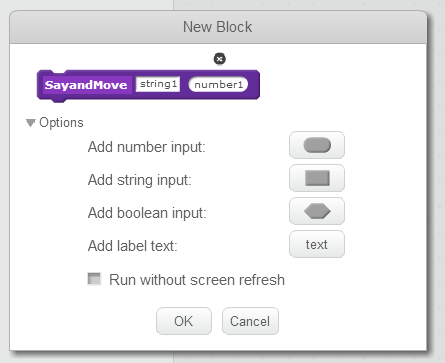
\includegraphics[width=6cm]{fig/makeBlockSmall.png}
  \caption{}
  \label{fig:makeBlock}
  \end{center}
\end{figure} 

\begin{figure}
  \begin{center}
  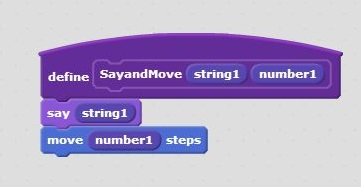
\includegraphics[width=6cm]{fig/useBlockSmall.png}
  \caption{}
  \label{fig:useBlock}
  \end{center}
\end{figure} 




\section{Dataset}
\label{dataset}
We scraped all Scratch programs uploaded \todo{add date range?} from the Scratch website with a scraping program. This resulted in he JSON code for \nPrograms~Scratch programs. In addition to the programs themselves, we also gathered metadata including the numbers of views, loves, favorites and remixes. Out of the \nPrograms~, we failed to analyze 2.367 programs due to various technical difficulties \todo{add details?} 

\subsection{Empty programs}

Also, interestingly enough, \nemptyPrograms~were empty (5.7\%), at least in terms of scripts. So Scratch users were sharing program already that did not contain code yet. In some cases \todo{analyze too?} they contained scripts and costumes but no code and in others they were entirety empty apart from the Scratch cat added by default.

\subsection{Block Usage}

\subsection{Block Size}

\subsection{User-defined Blocks}

\subsection{Remixing}

\section{Clones Detection for Scratch programs}
\label{algo}
\label{clone_Detection}



\section{Results}
\label{results}
The overarching research question of this work is how common Scratch users clone in their programs. As explained in Section \ref{clone_Detection} we distinguish three different forms of clones: Exact clones within one sprite, exact clones between sprites of one program, clones of `wait' blocks.

\subsection{Exact clones within one sprite}

\subsection{Exact clones between sprites of one program}

\subsection{Clones of `wait' blocks}

This section presents the results of our clone detection algorithm on the \nScriptPrograms~ with scripts.



\section{Related Work}



\bibliographystyle{IEEEtran}
\bibliography{zotero}


\end{document}   
